\documentclass[review]{siamart190516}

% -----------------------------------------------------------------------------
% 1. Preamble and packages
\usepackage{amsfonts}
\usepackage{amsmath}
\usepackage{graphicx}
\usepackage{subfig}
\usepackage{epstopdf}
\usepackage{hyperref}
\ifpdf%
  \DeclareGraphicsExtensions{.eps,.pdf,.png,.jpg}
\else
  \DeclareGraphicsExtensions{.eps}
\fi
\usepackage{amsopn}
\DeclareMathOperator{\diag}{diag}
\usepackage{booktabs}

% Paper title
\newcommand{\TheTitle}{%
  Local Fourier Analysis of Balancing Domain Decomposition for High-Order Finite Element Operators
}

% Short title for running heads (if needed)
\newcommand{\TheShortTitle}{%
  LFA of BDDC for High-Order FEM
}

% Acknowledge funding or other resources
\newcommand{\TheFunding}{This work is supported by the Exascale Computing Project (17-SC-20-SC), a collaborative effort of two U.S. Department of Energy organizations (Office of Science and the National Nuclear Security Administration) responsible for the planning and preparation of a capable exascale ecosystem, including software, applications, hardware, advanced system engineering and early testbed platforms, in support of the nation’s exascale computing imperative.
}

% Authors: full names plus addresses.
\author{
  Jeremy L Thompson\thanks{Department of Applied Mathematics, University of Colorado, Boulder, CO
    (\email{jeremy@jeremylt.org}).}
  \and Jed Brown\thanks{Department of Computer Science, University of Colorado, Boulder, CO
    (\email{jed@jedbrown.org}).}
  \and Yunhui He\thanks{Department of Applied Mathematics, University of Waterloo, Waterloo, ON, Canada
    (\email{yunhui.he@uwaterloo.ca}).}
}
\newcommand{\TheShortAuthors}{
  J. L. Thompson, J. Brown, and Y. He
}

% Title and funding information on page
\title{{\TheTitle}\thanks{\TheFunding}}
\headers{\TheShortTitle}{\TheShortAuthors}

% Optional PDF information
\ifpdf
\hypersetup{
  pdftitle={\TheTitle},
  pdfauthor={\TheShortAuthors}
}
\fi
% -----------------------------------------------------------------------------

\begin{document}

\maketitle

\vspace{1cm}

% -----------------------------------------------------------------------------
\begin{abstract}
Domain decomposition methods are popular preconditioners for solving linear systems derived from discretizing PDEs.
Balancing Domain Decomposition by Constraints (BDDC) is a non-overlapping domain decomposition technique that is closely related to the dual primal version of finite element tearing and interconnecting.
Local Fourier Analysis (LFA) is a technique for investigating and tuning preconditioners for finite difference and finite element methods.
In this paper, we use LFAToolkit.jl, a Julia package for LFA of high-order finite element methods, to analyze BDDC for high-order finite elements.
Specifically, we develop LFA of BDDC with arbitrary second-order PDEs using high-order finite element discretizations and examine the performance of BDDC on subdomains consisting of single and multiple high-order finite elements.
We can replicate previous work on the LFA of BDDC on subdomains with multiple low-order elements.
Examples are presented in two and three dimensions to validate our LFA of BDDC for the Laplacian and linear elasticity.
\end{abstract}
% -----------------------------------------------------------------------------

% -----------------------------------------------------------------------------
\begin{keywords}
  % Keywords that describe the paper
  local Fourier analysis, BDDC, high-order, finite elements
\end{keywords}
% -----------------------------------------------------------------------------

% -----------------------------------------------------------------------------
\section{Introduction}\label{sec:intro}
% -----------------------------------------------------------------------------

Balancing Domain Decomposition by Constraints (BDDC) is a relatively new technique created by Dohrmann in 2003 \cite{dohrmann2003preconditioner}.
BDDC is an improvement upon balancing domain decomposition (BDD) \cite{mandel1993balancing}, which requires modifications to be effective for high-order problems, especially for three-dimensional problems.
The dual primal version of finite element tearing and interconnecting (FETI-DP) \cite{farhat2000scalable} is closely related to BDDC and the two are effectively the same technique, under certain assumptions \cite{mandel2007bddc}.

Domain decomposition techniques decompose the domain $\Omega$ into a series of subdomains $\Omega^i$.
Some techniques use overlapping subdomains, such as additive Schwartz methods, which are popular for high-order and spectral finite elements \cite{fischer1997overlapping} and have been used as smoothers in multigrid methods \cite{fischer2005hybrid}.
In BDDC, we instead use non-overlapping subdomains with an energy minimization problem to resolve jumps in the values of degrees of freedom over subdomain interfaces.

LFA of BDDC was introduced by Brown, He, and MacLachlan \cite{brown2019local}.
We will discuss implementing BDDC in a matrix-free fashion and re-derive the LFA of BDDC in the context of high-order elements, with single element and macro-element subdomains.

This paper is organized as follows.
In \cref{sec:notation} we outline the notation for LFA used in this paper.
In \cref{sec:lfa} we develop the notation for LFA of second-order PDEs with arbitrary order bases, dimension, and number of components used in LFAToolkit.jl, and we use this notation to develop LFA of BDDC.
\Cref{sec:results} contains numerical results investigating the performance of BDDC on high and low-order elements for the two dimensional scalar Laplacian and three dimensional linear elasticity.
Finally, \cref{sec:conclusion} contains concluding remarks.

% -----------------------------------------------------------------------------
\subsection{Reproducibility}\label{sec:reproducibility}
% -----------------------------------------------------------------------------

The numerical results for LFA in this paper were generated using the Julia package LFAToolkit.jl \cite{thompson2021toolkit}.
This package is under active development and may be found on GitHub at \href{https://github.com/jeremylt/LFAToolkit.jl}{jeremylt/LFAToolkit.jl}.
This repository contains Julia scripts and interactive Jupyter notebooks that can replicate the tables and plots in this paper.

% -----------------------------------------------------------------------------
\section{Definitions and Notation}\label{sec:notation}
% -----------------------------------------------------------------------------

Consider a scalar Toeplitz operator $L_h$ on an infinite one dimensional uniform nodal grid $G_h$,
\begin{equation}
\begin{split}
L_h \mathrel{\hat{=}} \left[ s_\kappa \right]_h \left( \kappa \in V \right);\\
L_h w_h \left( x \right) = \sum_{\kappa \in V} s_\kappa w_h \left( x + \kappa h \right),
\end{split}
\end{equation}
where $V \subset \mathbb{Z}$ is a finite index set, $s_\kappa \in \mathbb{R}$ are constant coefficients, and $w_h \left( x \right)$ is a $l^2$ function on $G_h$. In the terminology of stencils, $s_{\kappa}$ are stencil weights that are nonzero on the neighborhood $\kappa \in V$.

Since $L_h$ is Toeplitz, it can be diagonalized by the standard Fourier modes $\varphi \left( \theta, x \right) = e^{\imath \theta x / h}$, which alias according to $\varphi(\theta+ 2\pi/h, x) = \varphi(\theta, x)$ on all grid points $x \in h \mathbb Z$.

\begin{definition}[Symbol of $L_h$]\label{def:symbol}
If for all grid functions $\varphi \left( \theta, x \right)$ we have
\begin{equation}
L_h \varphi \left( \theta, x \right) = \tilde{L}_h \left( \theta \right) \varphi \left( \theta, x \right),
\end{equation}
then we define $\tilde{L}_h \left( \theta \right) = \sum_{\kappa \in V} s_\kappa e^{\imath \theta \kappa}$ as the symbol of $L_h$, where $\imath^2 = -1$.
\end{definition}

This definition can be extended to a $q \times q$ linear system of operators by
\begin{equation}
\mathbf{L}_h =
\begin{bmatrix}
    L_h^{1, 1} && \cdots && L_h^{1, q}        \\
    \vdots               && \vdots && \vdots  \\
    L_h^{q, 1} && \cdots && L_h^{q, q}        \\
\end{bmatrix},
\end{equation}
where $L_h^{i, j}$, $i, j \in \lbrace 1, 2, \dots, q \rbrace$ are given by scalar Toeplitz operators describing how component $j$ appears in the equation for component $i$.
The components here may represent different fields and/or nodes of a finite element basis.
The symbol of $\mathbf{L}_h$, denoted $\tilde{\mathbf{L}}_h$, is a $q \times q$ matrix-valued function of $\theta$ given by $\left( \tilde{\mathbf{L}}_h \right)_{i, j} = \tilde{L}_h^{i, j} \left( \theta \right)$.
For a system of equations representing an error propagation operator in a relaxation scheme, the spectral radius of the symbol matrix determines how rapidly the scheme decreases error at a target frequency.

These definitions are readily extended to $d$ dimensions by taking the neighborhood $V \subset \mathbb Z^d$ and letting $\theta \in [-\pi,\pi)^d$.
For standard coarsening from fine $h=1$ to coarse $h=2$, low frequencies are given by $\theta \in T^{\text{low}} = \left[ - \pi / 2, \pi / 2 \right)^d$ and high frequencies are given by $\theta \in \left[-\pi, \pi \right)^d \setminus T^{\text{low}}$ or equivalently by periodicity, $\theta \in T^{\text{high}} = \left[ - \pi / 2, 3 \pi / 2 \right)^d \setminus T^{\text{low}}$.

% -----------------------------------------------------------------------------
\section{Local Fourier Analysis for Balancing Domain Decomposition by Constraints}\label{sec:lfa}
% -----------------------------------------------------------------------------

We now describe the LFA formulation used in LFAToolkit.jl and develop LFA of BDDC with high-order finite elements.

% -----------------------------------------------------------------------------
\subsection{High-Order Finite Elements}\label{sec:highorder}
% -----------------------------------------------------------------------------

We will use the representation of the weak form of linear second-order PDEs described in \cite{brown2010efficient}, which is given by
\begin{equation}
\langle v, f \left( u \right) \rangle = \int_{\Omega}
\begin{bmatrix}
  v^T & \nabla v^T    \\
\end{bmatrix}
\begin{bmatrix}
  f_{0, 0} & f_{0, 1} \\
  f_{1, 0} & f_{1, 1} \\
\end{bmatrix}
\begin{bmatrix}
  u                   \\
  \nabla u            \\
\end{bmatrix}
= \int_{\Omega} f v,\quad \forall v \in \mathcal V
\end{equation}
for some suitable $\mathcal V \subseteq H_0^1 \left( \Omega \right)$.
In this equation, $f_{i, j}$ may come from a linear PDE or the linearization of a non-linear problem.
Boundary terms have been omitted, as they are not present on the infinite uniform grid $G_h$.

Selecting a finite element basis, we can discretize this weak form and produce
\begin{equation}\label{eq:pdediscrete}
\mathbf{A} \mathbf{u} = \mathbf{b}.
\end{equation}

Using the algebraic representation of PDE operators given in \cite{brown2010efficient}, the PDE operator $\mathbf{A}$ is of the form
\begin{equation}\label{efficienthighorder}
\mathbf{A} = \mathbf{G}^T \mathbf{A}_e \mathbf{G},\quad \text{with} \,\,\mathbf{A}_e = \mathbf{B}^T \mathbf{D} \mathbf{B},
\end{equation}
where $\mathbf{G}$ represents the element assembly operator, $\mathbf{B}$ is a basis operator which computes the values and derivatives of the basis functions at the quadrature points, and $\mathbf{D}$ is a block diagonal operator which provides the pointwise application of the bilinear form on the quadrature points, to include quadrature weights and the change in coordinates between the physical and reference space.

\begin{definition}\label{def:high_order_symbol}
The symbol matrix of a finite element operator for an arbitrary second order PDE with any basis order, dimension, and number of components is given by
\begin{equation}\label{symbolhighorder}
\tilde{\mathbf{A}} = \mathbf{Q}^T \left( \mathbf{A}_e \odot \left[ e^{\imath \left( \mathbf{x}_j - \mathbf{x}_i \right) \cdot \boldsymbol{\theta} / \mathbf{h}} \right] \right) \mathbf{Q},
\end{equation}
where $\odot$ represents pointwise multiplication of the elements, $\mathbf{h}$ is the length of the element in each dimension, $\boldsymbol{\theta}$ is the target frequency in each dimension, $i, j \in \lbrace 1, 2, \dots, n \cdot \left( p + 1 \right)^d \rbrace$, $n$ is the number of components, $p$ is the polynomial degree of the discretization, and $d$ is the dimension of the finite element basis.
$\mathbf{A}_e$ is the finite element operator for the element and $\mathbf{Q}$ is the localization of Fourier modes on an element.
\end{definition}

Note that this LFA notation is applicable to any second-order PDE with a weak form that can be represented by \cref{efficienthighorder}.
This representation is used in LFAToolkit.jl, where the users provide the finite element basis $\mathbf{B}$, the node to mode localization operator $\mathbf{Q}$, and the pointwise representation of the weak form $\mathbf{D}$, and the software can provide the LFA of the PDE with various preconditioners.
The nodes may be defined by points $\mathbf x_i$ or more generally, as dual basis functions that may be applied to the Fourier modes; however, we restrict ourselves to nodal bases in this paper.
For further details, see CITATION TO THE FIRST PAPER.

% -----------------------------------------------------------------------------
\subsection{Balancing Domain Decomposition by Constraints}\label{sec:lfabddc}
% -----------------------------------------------------------------------------

With this representation of the symbol of high-order PDE operators, we can derive the symbol of BDDC preconditioned operators.

For high-order matrix-free BDDC, we decompose the domain $\Omega$ into a series of subdomains $\Omega^e$ given by the individual elements, and we utilize four non-exclusive spaces on each subdomain.
Figure \ref{fig:bddc_mesh_not_decomposed} shows a global mesh before decomposition, consisting of four quadratic elements in two dimensions, in this example.

The interface between subdomains is given by $\Gamma = \bigcup \partial \Omega^e \backslash \partial \Omega$ and the interface of subdomain $\Omega^e$ is given by $\Gamma^e = \delta \Omega^e \bigcap \Gamma$.
The interior of each subdomain, $\text{I}$, is given by the remaining degrees of freedom on the element.
In \cref{fig:bddc_mesh_interface}, the interface degrees of freedom, $\Gamma$, for each subdomain have been highlighted and the interior $\text{I}$ is given by the remainder of each subdomain.

\begin{figure}[!ht]
  \centering
  \subfloat[Global Problem Mesh]{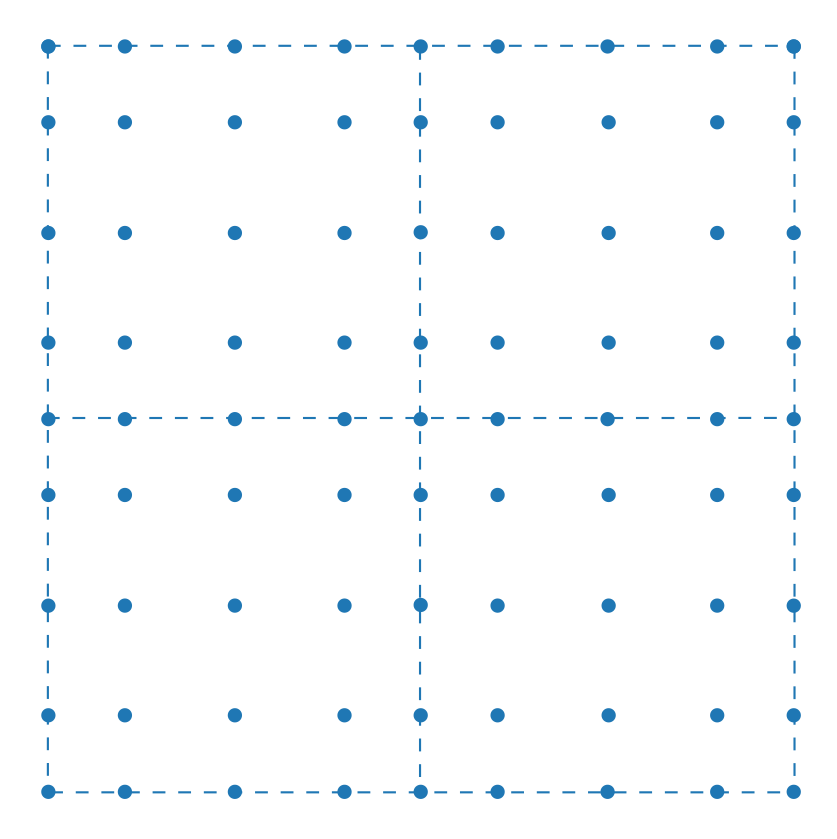
\includegraphics[width=0.48\textwidth]{img/HighOrderBDDCMesh}\label{fig:bddc_mesh_not_decomposed}}
  \hfill
  \subfloat[Subdomain Interfaces]{\includegraphics[width=0.48\textwidth]{img/HighOrderBDDCMeshInterface}\label{fig:bddc_mesh_interface}}\\
  \subfloat[BDDC Primal Nodes]{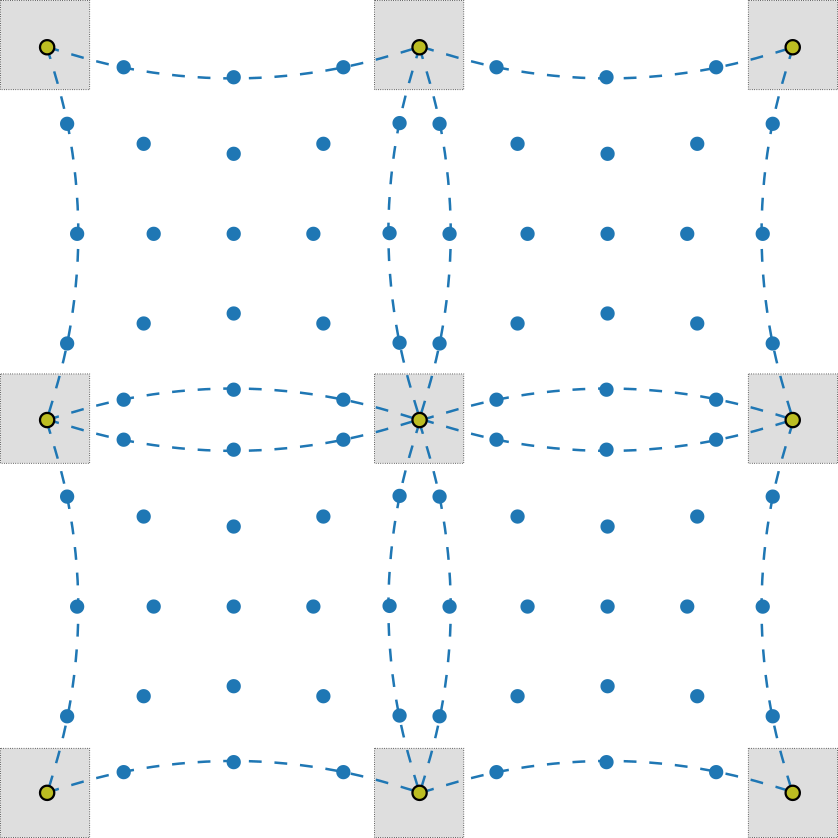
\includegraphics[width=0.48\textwidth]{img/HighOrderBDDCMeshPrimal}\label{fig:bddc_mesh_primal}}
  \hfill
  \subfloat[BDDC Duplicated Interface Nodes]{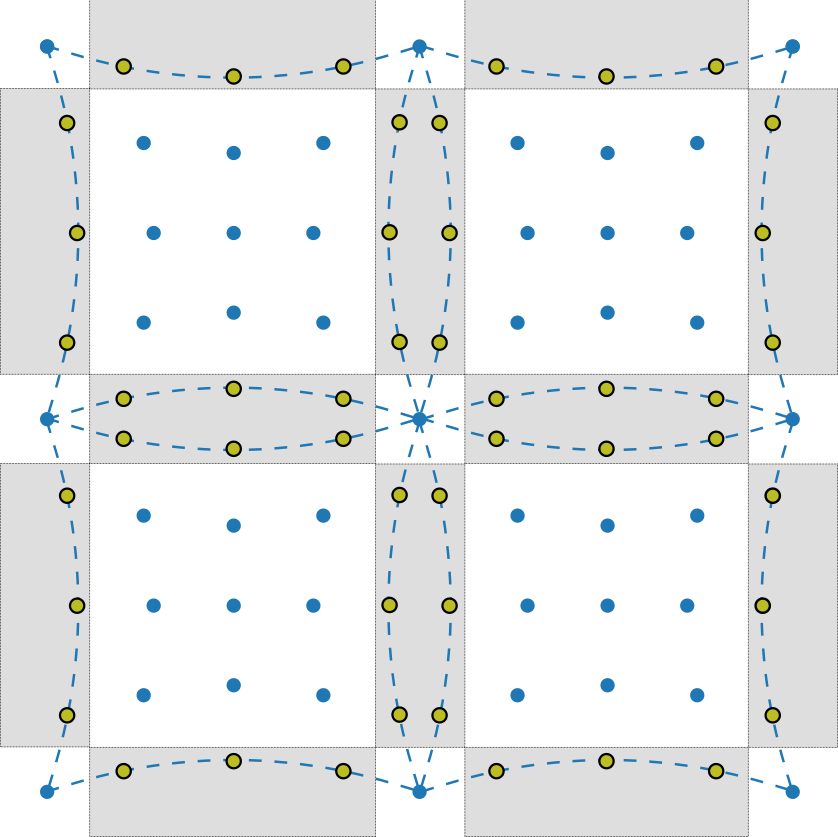
\includegraphics[width=0.48\textwidth]{img/HighOrderBDDCMeshInterfaceBroken}\label{fig:bddc_mesh_broken_interface}}
  \caption{Non-Overlapping Decomposition of Domain for BDDC.}
\end{figure}

Each subdomain problem could therefore be written as
\begin{equation}
\mathbf{A}^e =
\left[ \begin{array}{c c}
\mathbf{A}_{\text{I}, \text{I}}^e  &  \mathbf{A}_{\Gamma, \text{I}}^{e, T}  \\
\mathbf{A}_{\Gamma, \text{I}}^e    &  \mathbf{A}_{\Gamma, \Gamma}^e         \\
\end{array} \right]
\end{equation}
where $\mathbf{A}^e = \mathbf{B}^T \mathbf{D} \mathbf{B}$, as shown in Equation \ref{eq:pdediscrete}.

This subdomain problem can be assembled into the global problem in the typical finite element approach given by \cref{eq:pdediscrete}, but in BDDC we create a partially subassembled problem that is easier to invert than the global problem by duplicating broken degrees of freedom along the subdomain boundaries.
Only the corner, or vertex, degrees of freedom from each element are assembled into a global coarse problem while the remaining degrees of freedom on the subdomain interfaces are duplicated in each subdomain.
The solutions on the global coarse problem and broken subdomain problems are used to construct an approximate solution to the true assembled global problem.

The coarse grid, or primal, nodes $\Pi^e$ are given by the corners of the subdomain, so we have $4$ primal nodes for each element in two dimensions and $8$ primal nodes in three dimensions.
The remainder of the subdomain we denote with an $\text{r}$.
In \cref{fig:bddc_mesh_primal} the primal nodes have been highlighted.

The partially subassembled problem is therefore given by
\begin{equation}
\hat{\mathbf{A}} = \sum_{e = 1}^N \mathbf{R}^{e, T} \hat{\mathbf{A}}^e \mathbf{R}^e
\label{eq:subassembled}
\end{equation}
where
\begin{equation}
\hat{\mathbf{A}}^e =
\left[ \begin{array}{c c}
\mathbf{A}_{\text{r}, \text{r}}^e  &  \hat{\mathbf{A}}_{\Pi, \text{r}}^{e, T}  \\
\hat{\mathbf{A}}_{\Pi, \text{r}}^e   &  \hat{\mathbf{A}}_{\Pi, \Pi}^e           \\
\end{array} \right]
\end{equation}
and $\mathbf{R}^e$ is the subdomain injection operator. 
In this formulation, the broken degrees of freedom found on the portion of subdomain interface given by $\Gamma^e - \Pi^e$ are duplicated for each subdomain.
In \cref{fig:bddc_mesh_broken_interface} the duplicated degrees of freedom across each subdomain interface have been highlighted.
This duplication reduces the amount of global communication required to solve the subassemebled problem, which makes BDDC attractive as a preconditioner for high-order finite element methods.

There are BDDC formulations which enrich the primal space with edge or face averages to improve convergence.
We forgo these formulations to simplify the analysis; however these formulations can become increasingly attractive with large, high-order subdomains in three dimensions.
There is no fundamental barrier to extending the LFA of BDDC described below for formulations that use edge or face averages to improve convergence.

\begin{definition}\label{def:bddcpreconditioner}
The action of the BDDC preconditioner is given by
\begin{equation}
\mathbf{M}^{-1} = \mathbf{R}^T \hat{\mathbf{A}}^{-1} \mathbf{R}
\end{equation}
where $\mathbf{R}$ is the subassembly injection operator.
The inverse of the partially subassembled problem is computed by Schur complement
\begin{equation}
\hat{\mathbf{A}}^{-1} =
\left[ \begin{array}{c c}
\mathbf{I}  &  -\mathbf{A}_{\text{r}, \text{r}}^{-1} \hat{\mathbf{A}}_{\Pi, \text{r}}^T  \\
\mathbf{0}  &  \mathbf{I}                                                                \\
\end{array} \right]
\left[ \begin{array}{c c}
\mathbf{A}_{\text{r}, \text{r}}^{-1}  &  \mathbf{0}                   \\
\mathbf{0}                            &  \hat{\mathbf{S}}_{\Pi}^{-1}  \\
\end{array} \right]
\left[ \begin{array}{c c}
\mathbf{I}                                                              &  \mathbf{0}  \\
-\hat{\mathbf{A}}_{\Pi, \text{r}} \mathbf{A}_{\text{r}, \text{r}}^{-1}  &  \mathbf{I}  \\
\end{array} \right]
\end{equation}
where $\hat{\mathbf{S}}_{\Pi} = \hat{\mathbf{A}}_{\Pi, \Pi} - \hat{\mathbf{A}}_{\Pi, \text{r}} \mathbf{A}_{\text{r}, \text{r}}^{-1} \hat{\mathbf{A}}_{\Pi, \text{r}}^T$.
$\Pi$ denotes degrees of freedom on the assembled subdomain vertex space, while $r$ denotes degrees of freedom on the broken space given by the subdomain interior and duplicated portions of the subdomain interface.
\end{definition}

% -----------------------------------------------------------------------------
\subsubsection{Subassembled Symbol}\label{sec:lfasubassembled}
% -----------------------------------------------------------------------------

The symbol of the partially subassembled problem is delicate to compute because it requires both modes in the broken element space and the global primal variable space.
We will form the symbol of the three components of the partially subassembled problem, $\mathbf{A}_{r, r}^{-1}$, $\hat{\mathbf{S}}_{\Pi}^{-1}$, and $\hat{\mathbf{A}}_{\Pi, r}$, separately.

The Fourier modes on each broken element subdomain are separate, so the mode localization operator $\mathbf{Q}$ is not used for the symbol of the subdomain solver.
The subdomain solver is completely in the broken element space and therefore has a very straightforward symbol, given by
\begin{equation}
\tilde{\mathbf{A}}_{\text{r}, \text{r}}^{-1} \left( \boldsymbol{\theta} \right) = \mathbf{A}_{\text{r}, \text{r}}^{-1} \odot \left[ e^{\imath \left( \mathbf{x}_j - \mathbf{x}_i \right) \cdot \boldsymbol{\theta} / \mathbf{h}} \right]
\end{equation}
where $\mathbf{x}_i$ and $\mathbf{x}_j$ are the coordinates for the nodes in the partially subassembled space.

On the other hand, the Schur complement spans the entire primal space and requires the mode localization operator for the primal space $\mathbf{Q}_{\Pi}$.
The symbol of the Schur complement is given by
\begin{equation}
\tilde{\hat{\mathbf{S}}}_{\Pi}^{-1} \left( \boldsymbol{\theta} \right) = \left( \mathbf{Q}_{\Pi}^T \left( \hat{\mathbf{S}}_{\Pi} \odot \left[ e^{\imath \left( \mathbf{x}_j - \mathbf{x}_i \right) \cdot \boldsymbol{\theta} / \mathbf{h}} \right] \right) \mathbf{Q}_{\Pi} \right)^{-1}
\end{equation}
where $\mathbf{x}_i$ and $\mathbf{x}_j$ are the coordinates for the nodes in the primal space.
The primal vertex solve is global across the entire problem, so the corresponding Fourier modes are mapped to the global problem before being solved exactly.

For the mixed primal and subdomain operators, we use the Fourier mode localization only on the modes corresponding to the primal vertices, giving us
\begin{equation}
\tilde{\hat{\mathbf{A}}}_{\text{r}, \Pi} \left( \boldsymbol{\theta} \right) = \left( \hat{\mathbf{A}}_{\text{r}, \Pi} \odot \left[ e^{\imath \left( \mathbf{x}_j - \mathbf{x}_i \right) \cdot \boldsymbol{\theta} / \mathbf{h}} \right] \right) \mathbf{Q}_{\Pi}
\end{equation}
where $\mathbf{x}_i$ come from the partially subassembled space and $\mathbf{x}_j$ come from the primal variable space.

\begin{definition}[Symbol of Partially Subassembled Operator Inverse]
The symbol of the inverse of the partially subassembled problem is given by
\begin{equation}
\tilde{\hat{\mathbf{A}}}^{-1} =
\left[ \begin{array}{c c}
\mathbf{I}  &  -\tilde{\mathbf{A}}_{\text{r}, \text{r}}^{-1} \tilde{\hat{\mathbf{A}}}_{\Pi, \text{r}}^T  \\
\mathbf{0}  &  \mathbf{I}                                                                                                                             \\
\end{array} \right]
\left[ \begin{array}{c c}
\tilde{\mathbf{A}}_{\text{r}, \text{r}}^{-1}  &  \mathbf{0}                                        \\
\mathbf{0}                                                    &  \tilde{\hat{\mathbf{S}}}_{\Pi}^{-1}  \\
\end{array} \right]
\left[ \begin{array}{c c}
\mathbf{I}                                                                                                                           &  \mathbf{0}  \\
-\tilde{\mathbf{A}}_{\Pi, \text{r}} \tilde{\hat{\mathbf{A}}}_{\text{r}, \text{r}}^{-1}  &  \mathbf{I}  \\
\end{array} \right]
\end{equation}
In this notation, $\tilde{\mathbf{A}}$ indicates Fourier modes on the broken element space, while $\tilde{\hat{\mathbf{A}}}$ indicates Fourier modes on the global primal variable space.

The symbol of the subdomain solver is given by
\begin{equation}
\tilde{\mathbf{A}}_{\text{r}, \text{r}}^{-1} \left( \boldsymbol{\theta} \right) = \mathbf{A}_{\text{r}, \text{r}}^{-1} \odot \left[ e^{\imath \left( \mathbf{x}_j - \mathbf{x}_i \right) \cdot \boldsymbol{\theta} / \mathbf{h}} \right]
\end{equation}
while the symbol of the Schur complement solve is given by
\begin{equation}
\tilde{\hat{\mathbf{S}}}_{\Pi}^{-1} \left( \boldsymbol{\theta} \right) = \left( \mathbf{Q}_{\Pi}^T \left( \hat{\mathbf{S}}_{\Pi} \odot \left[ e^{\imath \left( \mathbf{x}_j - \mathbf{x}_i \right) \cdot \boldsymbol{\theta} / \mathbf{h}} \right] \right) \mathbf{Q}_{\Pi} \right)^{-1}
\end{equation}
and the symbol of the mixed primal and subdomain operators are given by
\begin{equation}
\tilde{\hat{\mathbf{A}}}_{\text{r}, \Pi} \left( \boldsymbol{\theta} \right) = \left( \hat{\mathbf{A}}_{\text{r}, \Pi} \odot \left[ e^{\imath \left( \mathbf{x}_j - \mathbf{x}_i \right) \cdot \boldsymbol{\theta} / \mathbf{h}} \right] \right) \mathbf{Q}_{\Pi}
\end{equation}
and $\tilde{\hat{\mathbf{A}}}_{\text{r}, \Pi}^T \left( \boldsymbol{\theta} \right)$ is given by the conjugate transpose.
The portion of the mode mapping operator on the primal nodes and modes is denoted $\mathbf{Q}_{\Pi}$.
The coordinates $\mathbf{x}_i$ and $\mathbf{x}_j$ are given in the partially subassembled space or primal space, as appropriate.
\label{def:subassembled_symbol}
\end{definition}

% -----------------------------------------------------------------------------
\subsubsection{Injection Symbols}\label{sec:lfainjection}
% -----------------------------------------------------------------------------

The injection operators map the global degrees of freedom to the partially subassembled spaces on each subdomain, and the symbols of the injection operators map the Fourier modes on the global space to the Fourier modes on the partially subassembled space.
We consider the two injection operators discussed by Brown, He, and MacLachlan in \cite{brown2019local}.

The first injection operator, $\mathbf{R}_1$, the scaled injection operator, results in the lumped BDDC preconditioner, $\mathbf{M}^{-1}_1$.

Let $\mathcal{N} \left( x \right)$ denote the set of subdomains that contain a broken copy of degree of freedom $x$ in the broken space.
If $x \in \Pi^e$ or $x \in \text{I}^e$, then $\lvert \mathcal{N} \left( x \right) \rvert = 1$, otherwise $\lvert \mathcal{N} \left( x \right) \rvert$ is the number of subdomains that contain $x$.
The scaled injection operator, $\mathbf{R}_1$ is defined as the mapping between the global degrees of freedom and the broken space where each element is scaled by $1 / \lvert \mathcal{N} \left( x \right) \rvert$.
For interior and vertex degrees of freedom, the sparse matrix representation of $\mathbf{R}_1$ would contain a single entry with a value of $1$, while each column corresponding to a duplicated degree of freedom has $\lvert \mathcal{N} \left( x \right) \rvert$ entries, each given by $1 / \lvert \mathcal{N} \left( x \right) \rvert$.

\begin{definition}[Scaled Injection Operator]
Let the scaled injection operator, $\mathbf{R}_1$, be given by the mapping from the global problem space to the broken space where each degree of freedom is scaled by its multiplicity in the broken space, denoted by $\lvert \mathcal{N} \left( x \right) \rvert$.
\label{def:scaledinjection}
\end{definition}

An operator preconditioned with the lumped BDDC preconditioner has the same eigenvalues as the lumped FETI-DP preconditioned operator, with the exception of some eigenvalues that are equal to $0$ and $1$ \cite{li2007use}.

The scaled injection operator, $\mathbf{R}_1$, is a pointwise scaling operator, so the operator is its own symbol.
We can partition $\mathbf{R}_1$ into its action on primal and subassembled nodes on each element,
\begin{equation}
\mathbf{R}_1^e =
\begin{bmatrix}
\mathbf{R}_{1, \Pi} &                    \\
                    & \mathbf{R}_{1, r}  \\
\end{bmatrix}.
\end{equation}

In the symbol of the subassembled inverse, the Fourier modes on the primal nodes have already been localized to Fourier modes in the global space, so we only need the Fourier mode localization operator on the subassembled nodes, denoted $\mathbf{Q}_r$.

\begin{definition}[Symbol of Scaled Injection Operator]
The symbol of the scaled injection operator is given by
\begin{equation}
\tilde{\mathbf{R}}_1 \left( \boldsymbol{\theta} \right) =
\begin{bmatrix}
\mathbf{I} &                    \\
           & \mathbf{R}_{1, r}  \\
\end{bmatrix}
\begin{bmatrix}
\mathbf{I} &                 \\
           & \mathbf{Q}_{r}  \\
\end{bmatrix}
\end{equation}
where $\mathbf{R}_{1, r}$ gives the portion of the scaled injection operator acting on the subassembled nodes and $\mathbf{Q}_r$ gives the portion of the Fourier mode localization operator that localizes the Fourier modes on the subassembled nodes.
\label{def:scaled_injection_symbol}
\end{definition}

The second injection operator, $\mathbf{R}_2$, the harmonic injection operator, results in the Dirichlet BDDC preconditioner, $\mathbf{M}^{-1}_2$.

This injection operator uses a discrete harmonic extension of the interface values to minimize the energy norm of the result, which leads to a better stability bound, as shown by Toselli and Widlund \cite{toselli2006domain}.
Let $\boldsymbol{\mathcal{H}}$ be given by a direct sum of local operators $\boldsymbol{\mathcal{H}}^e = - \mathbf{A}_{\text{I}, \text{I}}^{e, -1} \mathbf{A}_{\Gamma, \text{I}}^{e, T}$.
This operator solves a local Dirichlet problem given by mapping the jump over subdomain interfaces for duplicated values to the subdomain interior.

\begin{definition}[Harmonic Injection Operator]
Let the harmonic injection operator be given by $\mathbf{R}_2 = \mathbf{R}_1 - \mathbf{J}^T \boldsymbol{\mathcal{H}}^T$, where $\boldsymbol{\mathcal{H}}$ is given by a direct sum of local operators $\boldsymbol{\mathcal{H}}^e = - \mathbf{A}_{\text{I}, \text{I}}^{e, -1} \mathbf{A}_{\Gamma, \text{I}}^{e, T}$ and
\begin{equation}
\mathbf{J}^{e, T} v \left( x \right) = \sum_{i \in \mathcal{N} \left( x \right)} \left( \frac{v^e \left( x \right)}{\lvert \mathcal{N} \left( x \right) \rvert} - \frac{v^i \left( x \right)}{\lvert \mathcal{N} \left( x \right) \rvert} \right), \forall x \in \Gamma^e.
\end{equation}
\label{def:harmonicinjection}
\end{definition}

An operator preconditioned with the Dirichlet BDDC preconditioner, $\mathbf{M}^{-1}_2 \mathbf{A}$, has the same eigenvalues as the BDDC preconditioned operator with original formulation of the BDDC preconditioner given by Dohrmann \cite{dohrmann2003preconditioner}, with the exception of some eigenvalues that are equal to $1$ \cite{li2007use}.

For the symbol of the harmonic injection operator, we need the symbol of the harmonic extension and jump mapping.

As with the partially subassembled problem, the symbol of the harmonic extension is given by the symbols of the local operators.
The jump mapping is a pointwise scaling operator, so it is its own symbol, just as $\mathbf{R}_1$ is its own symbol.

\begin{definition}[Symbol of Harmonic Injection Operator]
The symbol of the harmonic injection operator is given by
\begin{equation}
\tilde{\mathbf{R}}_2 \left( \boldsymbol{\theta} \right) =
\begin{bmatrix}
\mathbf{I} &                                                                  \\
           & \mathbf{R}_{1, r} - \mathbf{J}^T_r \boldsymbol{\mathcal{H}}^T_r  \\
\end{bmatrix}
\begin{bmatrix}
\mathbf{I} &                 \\
           & \mathbf{Q}_{r}  \\
\end{bmatrix}
\end{equation}
where $\mathbf{R}_{1, r}$ gives the portion of the scaled injection operator acting on the subassembled nodes, $\mathbf{J}^T_r$ gives the portion of the jump mapping acting on the subassembled nodes, $\boldsymbol{\mathcal{H}}^T_r$ gives the portion of the harmonic extension acting on subassembled nodes, and $\mathbf{Q}_r$ gives the portion of the Fourier mode localization operator that localizes the Fourier modes on the subassembled nodes.

The symbol of the harmonic extension is given by the symbols of the local operators,
\begin{equation}
\tilde{\boldsymbol{\mathcal{H}}} = - \tilde{\mathbf{A}}_{I, I}^{-1} \tilde{\mathbf{A}}_{\Gamma, I}^T
\end{equation}
where
\begin{equation}
\tilde{\mathbf{A}}_{I, I}^{-1} \left( \boldsymbol{\theta} \right) = \mathbf{A}_{I, I}^{e, -1} \odot \left[ e^{\imath \left( \mathbf{x}_j - \mathbf{x}_i \right) \cdot \boldsymbol{\theta} / \mathbf{h}} \right],
\hspace{5mm}
\tilde{\mathbf{A}}_{\Gamma, I}^T \left( \boldsymbol{\theta} \right) = \mathbf{A}_{\Gamma, I}^{e, T} \odot \left[ e^{\imath \left( \mathbf{x}_j - \mathbf{x}_i \right) \cdot \boldsymbol{\theta} / \mathbf{h}} \right].
\end{equation}
The coordinates $\mathbf{x}_i$ and $\mathbf{x}_j$ are given in the subdomain interior or on subdomain interface, as appropriate.

The symbol of the jump mapping, $\tilde{\mathbf{J}}$, is a operator with entries on the diagonal given by
\begin{equation}
\tilde{\mathbf{J}}_{i, i} = - \frac{\lvert \mathcal{N} \left( x_i \right) \rvert - 1}{\lvert \mathcal{N} \left( x_i \right) \rvert}
\end{equation}
and off diagonal entries given by
\begin{equation}
\tilde{\mathbf{J}}_{i, j} = - \frac{1}{\lvert \mathcal{N} \left( x_i \right) \rvert} \hspace{2mm} \text{if} \hspace{2mm} x_j \in \mathcal{N} \left( x_i \right).
\end{equation}
\label{def:harmonic_injection_symbol}
\end{definition}

% -----------------------------------------------------------------------------
\subsubsection{BDDC Symbol}\label{sec:lfabddcsymbol}
% -----------------------------------------------------------------------------

The symbol of the lumped and Dirichled variants of BDDC are given by the symbol of the subassembled inverse and the respective injection operators.

\begin{definition}\label{def:bddc_symbol}
The symbol of the BDDC preconditioner is given by
\begin{equation}
\tilde{\mathbf{M}}^{-1}_i = \tilde{\mathbf{R}}^T_i \tilde{\hat{\mathbf{A}}}^{-1} \tilde{\mathbf{R}}_i
\end{equation}
where $\tilde{\mathbf{R}}_i$ is the symbol of the injection operator, given by \cref{def:scaled_injection_symbol,def:harmonic_injection_symbol}, and $\tilde{\hat{\mathbf{A}}}^{-1}$ is the symbol of the inverse of the subassembled problem, given by \cref{def:subassembled_symbol}.
\end{definition}

\begin{figure}[!tbp]
  \centering
  \subfloat[Spectrum of Lumped BDDC for $p = 4$]{\includegraphics[width=0.48\textwidth]{img/LumpedBDDCHighOrder}\label{fig:lumped_spectrum_4}}
  \hfill
  \subfloat[Spectrum of Dirichlet BDDC for $p = 4$]{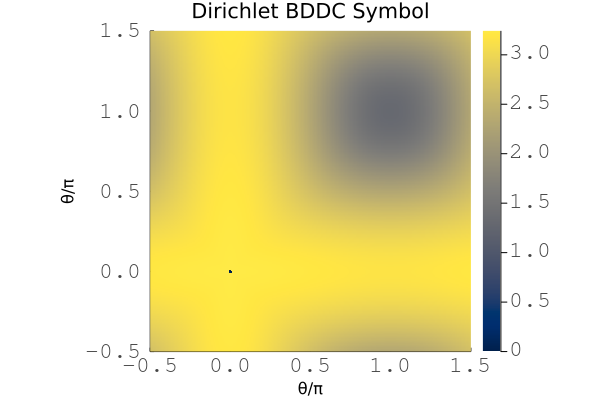
\includegraphics[width=0.48\textwidth]{img/DirichletBDDCHighOrder}\label{fig:dirichlet_spectrum_4}}
  \caption{BDDC preconditioning for high-order finite elements for the 2D Laplacian.}
\end{figure}

Using \cref{def:bddc_symbol}, we plot the spectral radius of $\tilde{\mathbf{M}}^{-1}_i \tilde{\mathbf{A}} \left( \boldsymbol{\theta} \right)$ in \cref{fig:lumped_spectrum_4,fig:dirichlet_spectrum_4} for the lumped and Dirichlet BDDC preconditioned operator, respectively, for the two dimensional Laplacian with a 4th degree $H^1$ Lagrange basis functions on Gauss-Lobatto points.
As anticipated, the Dirichlet BDDC preconditioner more effectively reduces the condition number of the two dimensional Laplacian than the Lumped BDDC preconditioner.

% -----------------------------------------------------------------------------
\section{Numerical Results}\label{sec:results}
% -----------------------------------------------------------------------------

In this section, we present validation with previous numerical results for this analysis for the scalar Laplacian in two dimensions with $H^1$ Lagrange bases on Gauss-Lobatto points with Gauss-Legendre quadrature.

% -----------------------------------------------------------------------------
\subsection{Scalar Laplacian - Low-Order Validation}\label{sec:lowordervalidate}
% -----------------------------------------------------------------------------

By using macro-elements, \cite{kumar2019local, brown2019local}, our LFA of BDDC on subdomains consisting of single high-order elements can be extended to subdomains consisting of multiple elements.
For 1D analysis, a macro-element for a two element subdomain is single element comprising of a pair of sub-elements with separate quadrature spaces, which is equivalent to partially assembling the finite element operator on two element subdomains.

Previous work by Brown, He, and MacLachlan \cite{brown2019local} provided LFA of lumped and Dirichlet BDDC on subdomains consisting of multiple low-order finite elements.
This previous work provided very sharp LFA convergence estimates when compared to numerical experiments with PETSc \cite{petsc-user-ref} on a periodic mesh.
Our LFA of BDDC can reproduce this previous work with macro-elements consisting of multiple linear elements.

\begin{table}[ht!]
\begin{center}
\begin{tabular}{l ccc ccc}
  \toprule
  $m$  &  \multicolumn{3}{c}{Lumped BDDC}  &  \multicolumn{3}{c}{Dirichlet BDDC}  \\
  %\cmidrule(lr){2-3} \cmidrule(lr){4-5} \cmidrule(lr){6-7}
                      &  $\lambda_{\min}$  &  $\lambda_{\max}$  &  $\kappa$ & $\lambda_{\min}$  &  $\lambda_{\max}$ & $\kappa$  \\
  \toprule
  $m = 4$   &  1.000  &   4.444  &   4.444  &  1.000  &  2.351  &  2.351  \\
  $m = 8$   &  1.000  &  12.269  &  12.269  &  1.000  &  3.196  &  3.196  \\
  $m = 16$  &  1.000  &  31.179  &  31.179  &  1.000  &  4.188  &  4.188  \\
  $m = 32$  &  1.000  &  75.761  &  75.761  &  1.000  &  5.335  &  5.335  \\
  \bottomrule
\end{tabular}
\end{center}
\caption{Condition Numbers and Maximal Eigenvalues for Low-Order Macro-Element Subdomains.}
\label{table:macro_element_bddc}
\end{table}

\cref{table:macro_element_bddc} shows the maximal eigenvalues and condition numbers for the symbol of the BDDC preconditioned operator $\tilde{\mathbf{M}}^{-1}_i \left( \boldsymbol{\theta} \right) \tilde{\mathbf{A}} \left( \boldsymbol{\theta} \right)$ for the two dimensional Poisson problem on linear macro-element subdomains with varying numbers of elements in one dimension.
The maximal eigenvalues were computed across $64$ uniformly spaced frequencies.
These values exactly agree with the previous work by Brown, He, and MacLachlan \cite{brown2019local}.

It is important to note the significantly improved condition number and resulting improved convergence for the Dirichlet BDDC.
Lumped BDDC has approximately half of the setup costs when compared to Dirichlet BDDC when using assembled exact inverses.
Brown, He, and MachLachlan investigated the use of multiplicative combinations of the lumped BDDC operator with a diagonal scaling operator to improve convergence while still retaining the benefit of cheaper setup for lumped BDDC.
This technique helped mitigate the growth of the condition number for the lumped BDDC as the subdomain size grew, but the resulting condition number was still larger than the condition number for Dirichlet BDDC.

% -----------------------------------------------------------------------------
\subsection{Scalar Laplacian - High-Order Validation}\label{sec:highordervalidate}
% -----------------------------------------------------------------------------

Single high-order elements can represent an equivalent number of degrees of freedom.
This approach has been investigated for solid mechanics problems, such as in \cite{pavarino2010bddc}; although, this work incorporated additional primal degrees of freedom from average values across subdomain edges and faces.

\begin{table}[ht!]
\begin{center}
\begin{tabular}{l ccc ccc}
  \toprule
  $p$  &  \multicolumn{3}{c}{Lumped BDDC}  &  \multicolumn{3}{c}{Dirichlet BDDC}  \\
                      &  $\lambda_{\text{min}}$  &  $\lambda_{\text{max}}$  &  $\kappa$ & $\lambda_{\text{min}}$  &  $\lambda_{\text{max}}$ & $\kappa$  \\
  \toprule
  $p = 2$   &  1.000  &    2.800  &    2.800  &  1.000  &  2.042  &  2.042  \\
  $p = 4$   &  1.000  &   12.948  &   12.948  &  1.000  &  3.242  &  3.242  \\
  $p = 8$   &  1.000  &   59.563  &   59.563  &  1.000  &  5.197  &  5.197  \\
  $p = 16$  &  1.000  &  289.678  &  289.678  &  1.000  &  7.761  &  7.761  \\
  \bottomrule
\end{tabular}
\end{center}
\caption{Condition Numbers and Maximal Eigenvalues for Single High-Order Element Subdomains.}
\label{table:high_order_element_bddc}
\end{table}

\cref{table:high_order_element_bddc} shows the maximal eigenvalues and condition numbers for the symbol of the BDDC preconditioned operator $\tilde{\mathbf{M}}^{-1}_i \left( \boldsymbol{\theta} \right) \tilde{\mathbf{A}} \left( \boldsymbol{\theta} \right)$ for the two dimensional Poisson problem on single high-order element subdomains with varying polynomial orders.

The improved condition number, and therefore convergence, of the Dirichlet BDDC compared to the lumped BDDC is more significant for high-order elements.
With single high-order element subdomains, the Fast Diagonalization Method approximate inverse subdomain solver can be used for both the subdomain subassembled inverse and subdomain interior inverse, which eliminates the advantage in reduced setup costs for lumped BDDC.

\begin{figure}[!ht]
  \centering
  \subfloat[Lumped BDDC]{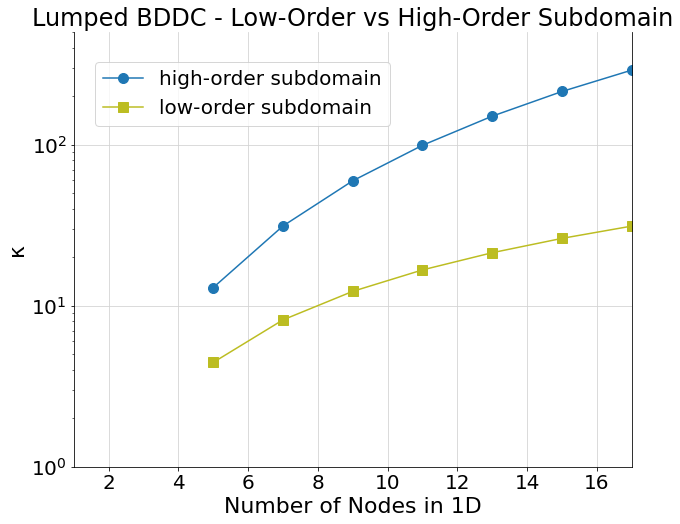
\includegraphics[width=0.48\textwidth]{img/lowVsHighLumped}\label{fig:lumped_bddc_comparison}}
  \hfill
  \subfloat[Dirichlet BDDC]{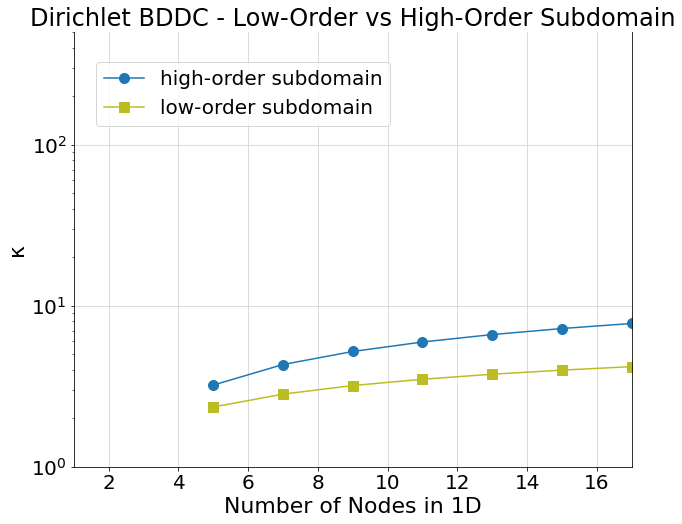
\includegraphics[width=0.48\textwidth]{img/lowVsHighDirichlet}\label{fig:dirichlet_bddc_comparison}}
  \caption{Low-Order and High-Order Subdomain Condition Number Comparison.}
\end{figure}

In \cref{fig:lumped_bddc_comparison} we compare the growth of the condition number for the lumped BDDC preconditioned operator for a subdomain consisting of several linear elements and a subdomain consisting of a single high-order element for the two dimensional Poisson problem.
The condition number grows much more rapidly for a high-order subdomain with an equivalent number of degrees of freedom.

In \cref{fig:dirichlet_bddc_comparison} we compare the growth of the condition number for the Dirichlet BDDC preconditioned operator for a subdomain consisting of several linear elements and a subdomain consisting of a single high-order element for the two dimensional Poisson problem.
In contrast with Figure \ref{fig:lumped_bddc_comparison}, we see that the condition number of the preconditioned operator on the high-order subdomain grows only slightly faster than the condition number of the low-order subdomain.

\begin{figure}[!ht]
  \centering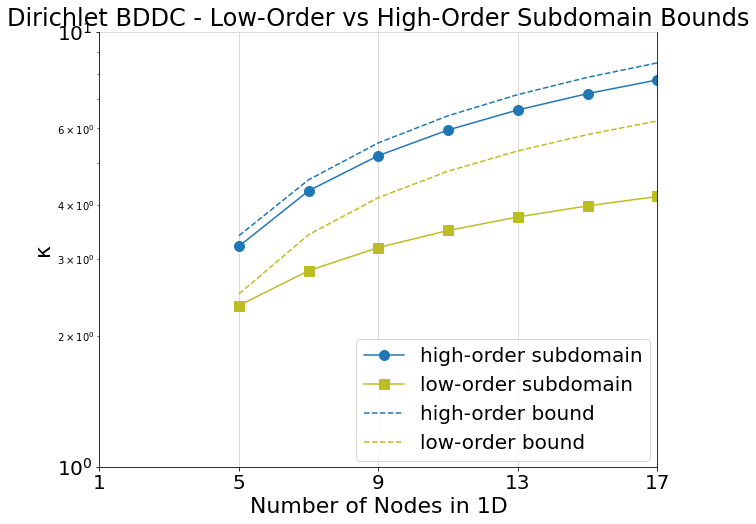
\includegraphics[width=0.48\textwidth]{img/lowVsHighDirichletBounds}
  \caption{Low-Order and High-Order Subdomain Condition Number Bounds.}
  \label{fig:dirichlet_bddc_bounds}
\end{figure}

The condition numbers of the Dirichlet BDDC preconditoner operator is bounded by
\begin{equation}
\kappa \leq \mathcal{C} \left( 1 + \log \left( p^2 \frac{H}{h} \right) \right)^2
\end{equation}
where $\mathcal{C} > 0$ is independent of the polynomial order $p$, the element size $h$, and the subdomain size $H$ \cite{klawonn2008spectral}.
In Figure \ref{fig:dirichlet_bddc_bounds}, we can see that our LFA-predicted condition numbers closely agree with this bound.

Klawonn, Pavarino, and Rheinbach investigated the performance of BDDC and FETI-DP preconditioners for the two dimensional Poisson problem with discontinuous coefficients \cite{klawonn2008spectral} and provided some experimentally derived maximal eigenvalues and condition numbers for the two dimensional Poisson problem.

\begin{table}[ht!]
\begin{center}
\begin{tabular}{l ccc ccc}
  \toprule
  $p$  &  \multicolumn{3}{c}{LFA}  &  \multicolumn{3}{c}{Experimental Results}  \\
                      &  $\lambda_{\text{min}}$  &  $\lambda_{\text{max}}$  &  $\kappa$ & $\lambda_{\text{min}}$  &  $\lambda_{\text{max}}$ & $\kappa$  \\
  \toprule
  $p = 2$   &  1.000  &   2.042  &   2.042  &  1.001  &   1.66  &   1.66  \\
  $p = 3$   &  1.000  &   2.614  &   2.614  &  1.000  &   2.38  &   2.38  \\
  $p = 4$   &  1.000  &   3.241  &   3.241  &  1.001  &   3.03  &   3.03  \\
  $p = 8$   &  1.000  &   5.195  &   5.194  &  1.001  &   5.01  &   5.00  \\
  $p = 16$  &  1.000  &   7.756  &   7.756  &  1.001  &   7.62  &   7.61  \\
  $p = 32$  &  1.000  &  10.961  &  10.961  &  1.002  &  10.86  &  10.84  \\
  \bottomrule
\end{tabular}
\end{center}
\caption{Condition Numbers and Maximal Eigenvalues for Dirichlet BDDC with Single Element High-Order Subdomains.}
\label{table:high_order_bddc_experiments_1}
\end{table}

\begin{table}[ht!]
\begin{center}
\begin{tabular}{l ccc ccc}
  \toprule
  $p$  &  \multicolumn{3}{c}{LFA}  &  \multicolumn{3}{c}{Experimental Results}  \\
                      &  $\lambda_{\text{min}}$  &  $\lambda_{\text{max}}$  &  $\kappa$ & $\lambda_{\text{min}}$  &  $\lambda_{\text{max}}$ & $\kappa$  \\
  \toprule
  $p = 2$   &  1.000  &   2.700  &   2.700  &  1.001  &   2.33  &   2.33  \\
  $p = 3$   &  1.000  &   3.568  &   3.568  &  1.001  &   3.21  &   3.21  \\
  $p = 4$   &  1.000  &   4.305  &   4.305  &  1.002  &   4.00  &   3.99  \\
  $p = 8$   &  1.000  &   6.511  &   6.511  &  1.003  &   6.26  &   6.24  \\
  $p = 16$  &  1.000  &   9.354  &   9.354  &  1.002  &   9.16  &   9.14  \\
  $p = 32$  &  1.000  &  12.856  &  12.856  &  1.002  &  12.69  &  12.66  \\
  \bottomrule
\end{tabular}
\end{center}
\caption{Condition Numbers and Maximal Eigenvalues for Dirichlet BDDC 4 Element High-Order Subdomains.}
\label{table:high_order_bddc_experiments_2}
\end{table}

In \cref{table:high_order_bddc_experiments_1} we see the LFA-predicted maximal eigenvalues and condition numbers for the scalar Poisson problem in two dimensions with constant coefficients compared to numerical results on a domain with 576 subdomains consisting of a single high-order finite element.
The LFA-predicted condition numbers generally agree with the experimental results, typically providing a mildly pessimistic prediction when compared to the experimental results.

In \cref{table:high_order_bddc_experiments_1} we see the LFA-predicted maximal eigenvalues and condition numbers for the scalar Poisson problem in two dimensions with constant coefficients compared to numerical results on a domain with 576 subdomains consisting of four high-order finite elements.

% -----------------------------------------------------------------------------
\subsection{Linear Elasticity - 3D Convergence Factors}\label{sec:solidsresults}
% -----------------------------------------------------------------------------

ToDo

% -----------------------------------------------------------------------------
\section{Conclusions}\label{sec:conclusion}
% -----------------------------------------------------------------------------

In this paper we developed LFA of BDDC with arbitrary second-order PDEs using high-order finite element discretizations by using an operator representation for efficient application of matrix-free implementations.
We used LFAToolkit.jl to investigate BDDC on high-order elements and validate against previous work.

The LFA of BDDC framework presented here can be extended to the LFA of BDDC on low-order finite elements and reproduces previous work in this area and agrees with condition numbers from previous work on LFA of BDDC for high-order finite elements.

% -----------------------------------------------------------------------------
\bibliographystyle{siamplain}
\bibliography{../references}
% -----------------------------------------------------------------------------

\end{document}

% -----------------------------------------------------------------------------
